\newpage
\section{Google API Service Implementation}
    Following the design in the section \ref{ssec:srp} the class 
    GoogleAPIService is responsible to make the request to the Google
    Direction API and return the result to the presenter which will be
    processed by the I/O service. The fig \ref{fig:directionServiceSeqDiagram}
    describes the object interactions and the messages exchanged during the
    single request that is made in order to receive a navigation data as described in
    the list \ref{code: googleAPi Result}.
    
    \par
        The GoogleDirectionAPIService implementation can be seen in
        the appendix \ref{code:googleAPIService}.
        Dependencies for the realizations are described below:
        \begin{enumerate}
            \item  
                \textbf{AsyncTaskUtil}
                    This is a custom made class which is reusable and used for background
                    operations see appendix \ref{code:AsyncUtil}. It is used here to make an HTTP request and this enables
                    the task to run without blocking the main thread. 
            \item  
                \textbf{GoogleDirectionApiMiddleware}
                As described earlier to make http request a HTTP client 
                is required and Retrofit
                is being used. Some parameters like the base endpoint of googleAPI 
                (where the http
                request would be made. i.e. https://maps.googleapis.com/), 
                connection and read timeouts
                to ensure the request is terminated 
                in case of situation when the server is not available 
                and error handling methods are configured in 
                GoogleDirectionMiddleware. Please see the appendix 
                \ref{code:retrofitConfig} to check the configuration. 
            \item  
                \textbf{DirectionAPI}
                    This is the model of the returned result from the Google
                    API.
            \item  
                \textbf{IAsyncTaskListenerOnFinish}
                    This is the listener which would get triggered when the
                    async task (HTTP request to Google API here) completes to
                    return the result.
        \end{enumerate}       
        



    \begin{figure}[htbp!]
        \centering 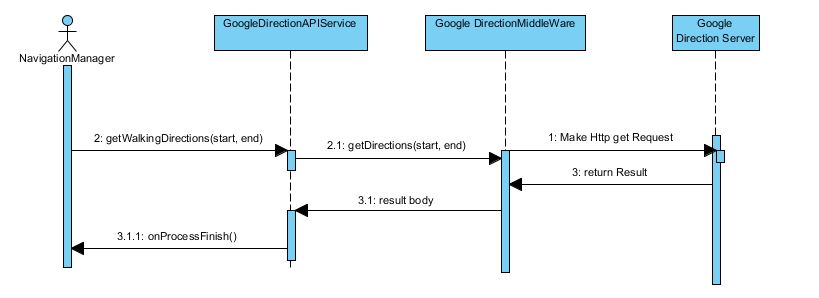
\includegraphics[scale=0.75]{grafiken/seqDigGoogleAPI.jpg}
        \caption{Sequence Diagram: Describing the functonality of the Google API service}
        \label{fig:directionServiceSeqDiagram}
    \end{figure}